% 
% Annual Cognitive Science Conference
% Sample LaTeX Paper -- Proceedings Format
% 

% Original : Ashwin Ram (ashwin@cc.gatech.edu)       04/01/1994
% Modified : Johanna Moore (jmoore@cs.pitt.edu)      03/17/1995
% Modified : David Noelle (noelle@ucsd.edu)          03/15/1996
% Modified : Pat Langley (langley@cs.stanford.edu)   01/26/1997
% Latex2e corrections by Ramin Charles Nakisa        01/28/1997 
% Modified : Tina Eliassi-Rad (eliassi@cs.wisc.edu)  01/31/1998
% Modified : Trisha Yannuzzi (trisha@ircs.upenn.edu) 12/28/1999 (in process)
% Modified : Mary Ellen Foster (M.E.Foster@ed.ac.uk) 12/11/2000
% Modified : Ken Forbus                              01/23/2004
% Modified : Eli M. Silk (esilk@pitt.edu)            05/24/2005
% Modified: Niels Taatgen (taatgen@cmu.edu) 10/24/2006

%% Change ``a4paper'' in the following line to ``letterpaper'' if you are
%% producing a letter-format document.

\documentclass[10pt,letterpaper]{article}

\usepackage{mathtools}
\usepackage{cogsci}
\usepackage{pslatex}
\usepackage{apacite}


\title{Using Regular Expressions to Define String Groups}
 
\author{{\large \bf{P. Thomas Barthelemy} (bartho@stanford.edu)} \\
  Department of Computer Science, 353 Serra Mall \\
  Stanford, CA 94305 USA
  \AND {\large \bf Nicholas Borg (nickborg@stanford.edu)} \\
  Symbolic Systems Program, Margaret Jacks Hall \\
  Stanford, CA 94305 USA}


\begin{document}

\maketitle


\begin{abstract}
Regular expressions are used to define strings that match a certain pattern. In the following experiment, we posit that the means by which humans judge similarity of words can be represented by a method of inference using regular expressions. In short, there is a tradeoff of generality and specificity that allows for a selection of an optimal regular expression to categorize a list of input strings.

\textbf{Keywords:} 
Model inference, regular expression, anti-unification.
\end{abstract}


\section{Overview and Motivation}

\section{Inference over Regular Expressions}

\subsection{Balancing Generality with Specificity}
The goal of inference is to select a regular expression with the highest posterior probability. The posterior probability is proportional to the product of the hypothesis' prior probability and its likelihood.
\begin{align*}
	p(h|S) \propto p(h) p(S|h)
\end{align*}
Above, $S$ represents the set of input strings. We provide an equation for the prior probability such that our model biases smaller hypotheses, and the likelihood of generating a given hypothesis is inveresly proportional to its expressiveness. So, our model aims to balance generality with specificity.

\subsection{Hypothesis Representation: DFA}
Regular expressions are equivalent to deterministic finite automata (DFA).\footnote{See the Appendix for a brief summary of our regex notation.} DFA are often easier to reason with, and are thus used as the dominant representation for regexes throughout this paper.

To extract the likelihood of a hypothesis, probabilities are assigned to transitions. For our purposes, we assumed uniform probability across each potential transition. That is, in the regular exression \verb!a[b|c]!, $p(\verb!ab!)=p(\verb!ac!)=1/2$.

Further, we needed to define the probability with which a DFA would stop generating a string. For instance, given the regular expression \verb!a*!, we would need to define the probability of generating strings \verb!a!, \verb!aa!, \verb!aaa!, etc.

In this sense, our DFA is similar to a probabilistic automaton, although the acceptance criteria is $\tau=0$, so the languages represented by our DFA are still regular. [Citation]. A second difference is that there is no concept of stopping string generation in probabilistic automaton.

\subsection{Generating Hypotheses}
The hypothesis space is initiated with the base hypothesis, the term applied to a DFA that accepts strictly the input strings. Next, hypotheses are added to the hypothesis space through two processes of generalization: merging and applying wildcards.

\subsubsection{Merging} Merging is the process of combining states of a DFA. The newly create state has all incoming and outgoing transitions of its predecessors. Thus, the DFA will continue to accept the same set of strings as the original DFA. However, the DFA will often accept more strings after merging, thus merging states results in a more generalized DFA.

If merging is continued, the DFA will eventually have only one state with all transitions leading to itself. Such a state accepts all strings containing only zero or more of the original characters.

Because DFA have only one transition for any state and character, it is possible that merging two states will require further merging. This results in a chain-reaction of merging as shown in Figure~\ref{merge-figure}.

\begin{figure}[ht]
\begin{center}
\begin{align*}
\text{(a)}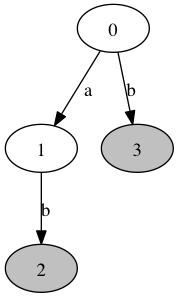
\includegraphics[scale=0.4]{merge-0.png}
&\text{(b)}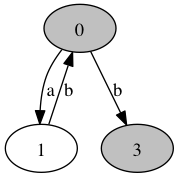
\includegraphics[scale=0.4]{merge-1.png}
&\text{(c)}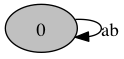
\includegraphics[scale=0.4]{merge-2.png}
\end{align*}
\end{center}
\caption{An example of state merging. The DFA starts at state 0 and accepts only at the shaded states. The base hypothesis accepts ``b'' and ``ab'' (a). After merging states 0 and 2, the next DFA accepts an infinite set of strings (b). Finally, the merge of states 0 and 1 forces the merge of state 0 and 3 to maintain one unique outbound transition for any state and character (c).} 
\label{merge-figure}
\end{figure}

[mention anti-unification]

\subsubsection{Wildcards} Wildcards generalize the DFA by extending state transitions to apply to a class of characters. The replacement of transition characters with wildcards might also cause chain merging, as shown in Figure~\ref{wildcard-figure}.

\begin{figure}[ht]
\begin{center}
\begin{align*}
\text{(a)}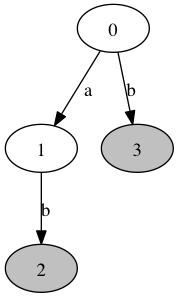
\includegraphics[scale=0.4]{wildcard-0.png}
&\text{(b)}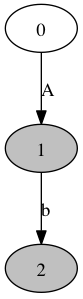
\includegraphics[scale=0.4]{wildcard-1.png}
\end{align*}
\end{center}
\caption{An example of inserting a wildcard, ``A'', which represents any character. Replacing a wildcard for one of the outbound transitions of state 0 has forced a merge of states 1 and 3.} 
\label{wildcard-figure}
\end{figure}

\subsection{Searching the Hypothesis Space} The number of hypotheses grows quickly with the number of states in the base hypothesis. As a lower bound, the number of hypotheses is at least as large as the number of possible starting nodes. Because the starting node could be merged with any subset of the remaining $n-1$ nodes in the DFA, there are $2^{n-1}=O(2^n)$ possible start states. Thus, the hypothesis space is at least exponential in the number of starting nodes in the regular expression.\footnote{See the Appendix for detailed sizing of the hypothesis space.}

\section{Inference with DFA}
\subsection{Prior Probability}
We assigned the prior probability to the hypotheses (i.e. regexes) based on the size of the DFA and the number of transitions. In the following equation, $|S|$ is the number of states in the DFA and $|T|$ is the number of tranisitons in the DFA, where a wildcard counts as only one transition. 
\begin{align*}
	P(h) \propto e^{-\alpha|S| - \beta|T|}
\end{align*}
Thus, we have biased smaller DFA that use wildcards instead of literal characters.

\subsection{Likelihood}
In assigning probabilities to state transitions and string acceptance, one can turn a DFA into a generative automaton. To simplify inference, we assume uniform probability over all possible state transitions. So, the probability of generating a string is simply the product of the transitions taken to arrive at that string. 

For the cases in which a string may alternatively be accepted or continue (e.g. \verb!ab*! can generate \verb!ab! or \verb!abb!), one must assign a probability for accepting or continuing the string. Let $\tau$ be the probability that the regex stops extending the string. Instead of leaving $\tau$ as a parameter of the model, we assume a uniform prior over the parameter and marginalize it when calculating the likelihood of a string. [citation]

\section{Experiment Design and Model Fitting}

\section{Results and Discussion}

\section{General Formatting Instructions}

For standard spoken papers and standard posters, the entire contribution (including figures, references, everything) can be no longer than six pages. For abstract posters, the entire contribution can be no longer than one page. For symposia, the entire contribution can be no longer than two pages.

The text of the paper should be formatted in two columns with an
overall width of 7 inches (17.8 cm) and length of 9.25 inches (23.5
cm), with 0.25 inches between the columns. Leave two line spaces
between the last author listed and the text of the paper. The left
margin should be 0.75 inches and the top margin should be 1 inch.
\textbf{The right and bottom margins will depend on whether you use
  U.S. letter or A4 paper, so you must be sure to measure the width of
  the printed text.} Use 10~point Times Roman with 12~point vertical
spacing, unless otherwise specified.

The title should be in 14~point, bold, and centered. The title should
be formatted with initial caps (the first letter of content words
capitalized and the rest lower case). Each author's name should appear
on a separate line, 11~point bold, and centered, with the author's
email address in parentheses. Under each author's name list the
author's affiliation and postal address in ordinary 10~point type.

Indent the first line of each paragraph by 1/8~inch (except for the
first paragraph of a new section). Do not add extra vertical space
between paragraphs.


\section{First-Level Headings}

First level headings should be in 12~point, initial caps, bold and
centered. Leave one line space above the heading and 1/4~ line space
below the heading.


\subsection{Second-Level Headings}

Second level headings should be 11~point, initial caps, bold, and
flush left. Leave one line space above the heading and 1/4~ line
space below the heading.


\subsubsection{Third-Level Headings}

Third-level headings should be 10~point, initial caps, bold, and flush
left. Leave one line space above the heading, but no space after the
heading.


\section{Formalities, Footnotes, and Floats}

Use standard APA citation format. Citations within the text should
include the author's last name and year. If the authors' names are
included in the sentence, place only the year in parentheses, as in
\citeA{NewellSimon1972a}, but otherwise place the entire reference in
parentheses with the authors and year separated by a comma
\cite{NewellSimon1972a}. List multiple references alphabetically and
separate them by semicolons
\cite{ChalnickBillman1988a,NewellSimon1972a}. Use the
et~al. construction only after listing all the authors to a
publication in an earlier reference and for citations with four or
more authors.


\subsection{Footnotes}

Indicate footnotes with a number\footnote{Sample of the first
  footnote.} in the text. Place the footnotes in 9~point type at the
bottom of the page on which they appear. Precede the footnote with a
horizontal rule.\footnote{Sample of the second footnote.}


\subsection{Tables}

Number tables consecutively; place the table number and title (in
10~point) above the table with one line space above the caption and
one line space below it, as in Table~\ref{sample-table}. You may float
tables to the top or bottom of a column, set wide tables across both
columns.

\begin{table}[!ht]
\begin{center} 
\caption{Sample table title.} 
\label{sample-table} 
\vskip 0.12in
\begin{tabular}{ll} 
\hline
Error type    &  Example \\
\hline
Take smaller        &   63 - 44 = 21 \\
Always borrow~~~~   &   96 - 42 = 34 \\
0 - N = N           &   70 - 47 = 37 \\
0 - N = 0           &   70 - 47 = 30 \\
\hline
\end{tabular} 
\end{center} 
\end{table}


\subsection{Figures}

All artwork must be very dark for purposes of reproduction and should
not be hand drawn. Number figures sequentially, placing the figure
number and caption, in 10~point, after the figure with one line space
above the caption and one line space below it, as in
Figure~\ref{sample-figure}. If necessary, leave extra white space at
the bottom of the page to avoid splitting the figure and figure
caption. You may float figures to the top or bottom of a column, or
set wide figures across both columns.

\begin{figure}[ht]
\begin{center}
\fbox{CoGNiTiVe ScIeNcE}
\end{center}
\caption{This is a figure.} 
\label{sample-figure}
\end{figure}


\section{Acknowledgments}

Place acknowledgments (including funding information) in a section at
the end of the paper.


\section{References Instructions}

Follow the APA Publication Manual for citation format, both within the
text and in the reference list, with the following exceptions: (a) do
not cite the page numbers of any book, including chapters in edited
volumes; (b) use the same format for unpublished references as for
published ones. Alphabetize references by the surnames of the authors,
with single author entries preceding multiple author entries. Order
references by the same authors by the year of publication, with the
earliest first.

Use a first level section heading for the reference list. Use a
hanging indent style, with the first line of the reference flush
against the left margin and subsequent lines indented by 1/8~inch.
Below are example references for a conference paper, book chapter,
journal article, technical report, dissertation, book, and edited
volume, respectively.

\nocite{ChalnickBillman1988a}
\nocite{Feigenbaum1963a}
\nocite{Hill1983a}
\nocite{OhlssonLangley1985a}
\nocite{Lewis1978a}
\nocite{NewellSimon1972a}
\nocite{ShragerLangley1990a}


\bibliographystyle{apacite}

\setlength{\bibleftmargin}{.125in}
\setlength{\bibindent}{-\bibleftmargin}

\bibliography{CogSci_Template}

\section{Appendix: Technical Notes}
\subsection{Regex and DFA Notation}
We used a limited alphabet wherein normal characters are all lower case. We also used the following rules to define regular expressions.
\begin{enumerate}
	\item Acceptance of specific strings is represented as concatenated characters. E.g. \verb!abc! accepts only \verb!abc!.
	\item Acceptance of disjunctive strings is represnted by \verb![a|b]!. E.g. \verb![abc|c]!accepts only \verb!abc! and \verb!c!.
	\item Acceptance of any character is represented by the wildcard \verb!?!. E.g. \verb!a?! accepts \verb!aa!, \verb!ab!, \verb!ac!, etc.
	\item Acceptance of the empty string is represented by \verb!E!. \verb!Ea! is the same as \verb!a!.
	\item Acceptance of any sequence repeated zero or more times is represented by the Kleene star, \verb!a*!. E.g. \verb!a*! accepts \verb!E!, \verb!a!, \verb!aa!, etc, 
\end{enumerate}

\subsection{Sizing the Hypothesis Space}
Ignoring wildcards and assuming that no chain-reaction merges occur, each hypothesis can be defined as a set of mutually exclusive subsets of the states contained in the base hypothesis. For instance, given states $s_1, s_2, s_3$, the possible hypotheses are:
	\begin{align*}
		&s_1, s_2, s_3
		\\&\text{merge}(s_1, s_2), s_3
		\\&\text{merge}(s_1, s_3), s_2
		\\&\text{merge}(s_2, s_3), s_1
		\\&\text{merge}(s_1, s_2, s_3)
	\end{align*}
To generalize this to a case of $n_b$ states in the base hypothesis, one can consider individually the number of regexes with $n_f$ states in the finished regex. For the cases where $n_b=n_f$ or $n_f=1$, it is easy to verify that there exist only one regex. When creating hypotheses where $1 < n_f < n_b$, however, one can simply look to the case of $n_b - 1$. In particular, for every $n_f$, one can simply duplicate all of the hypotheses from the $n_b - 1$ case with an additional unmerged state $s_{n_b}$. Further, one can add a new hypothesis for each subset of the hypotheses in the $n_s-1, n_f$ case. So, the expression for the total number of regexes given the number of states in the base hypothesis is given by $g(n_b)$.
	\begin{align*}
	f(a, b) &= \left\{
			\begin{array}{cl}
         		1 & a=b \vee b=1 \\
         		f(a-1, b-1) + b f(a-1, b) & \mbox{otherwise}
            \end{array}\right.
		\\ g(n_b) &=\sum_{n_f=1}^{n_b} f(n_b, n_f)
	\end{align*}
One of our experiment examples contained 25 nodes in the base hypothesis, which means that the hypothesis space is $g(25)\approx 5.0 \times 10^{17}$ regular expressions. Needless to say, it is intractable to exhaustively search the hypothesis space.

\end{document}
